\subsection{Measuring Congestion}\label{s:measurement}
\begin{figure}
    \centering
    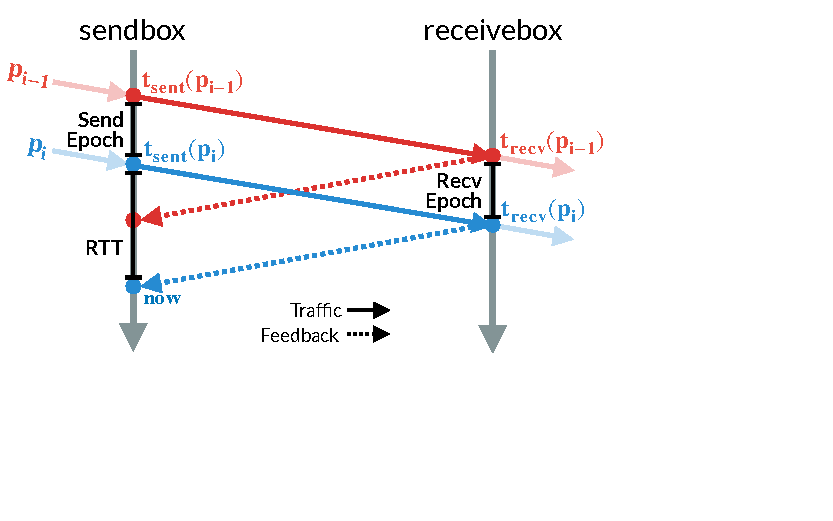
\includegraphics[width=\columnwidth]{img/rate-calculation}
    \caption{Example of epoch-based measurement calculation. Time moves from top to bottom.
    %Packets from flows in a bundle
    %pass through the \inbox and \outbox middleboxes on the way to their destination. 
    The \inbox records the packets that are identified as epoch boundaries. 
    The \outbox, up on identifying such packets, sends a feedback message back to
    the \inbox, which allows it to calculate the RTT and epochs.
    %When the \inbox observes a packet header matching the boundary condition, it records it. 
    %When the \outbox observes this packet, it sends an out-of-band feedback message back to
    %the \inbox, which allows it to calculate the RTT and epochs.
    }\label{fig:ratecalc}
\end{figure}

% \name uses out-of-band congestion ACKs to signal congestion between the \inbox and \outbox. 
% %Sending these congestion ACKs up on every packet is not just unnecessary, but also incurs high overhead. The \outbox instead sends congestion ACKs only for a few sampled packets. We refer to the period between two successively sampled packets as an \emph{epoch}, and each sampled packet as an \emph{epoch boundary packet}.
% We answer the following questions: (1) When should the \outbox send congestion ACKs? (2) What information should the congestion ACKs contain?

% \subsection{Timing of Congestion ACKs}
% \label{s:measure:marking}
% \newcommand{\pone}{$p_{i-1}$}
% \newcommand{\hpone}{$h(p_{i-1})$}
% \newcommand{\sone}{$s_{i-1}$}
% \newcommand{\rone}{$r_{i-1}$}
% \newcommand{\ptwo}{$p_{i}$}
% \newcommand{\hptwo}{$h(p_{i})$}
% \newcommand{\stwo}{$s_{i}$}
% \newcommand{\rtwo}{$r_{i}$}
% \newcommand{\atwo}{$a_{i}$}
% \newcommand{\sentone}{$sent_{i-1}$}
% \newcommand{\recvdone}{$rcvd_{i-1}$}
% \newcommand{\senttwo}{$sent_{i}$}
% \newcommand{\recvdtwo}{$rcvd_{i}$}

%\an{I think it would be possible to roll this into 4.5}
Sending an out-of-band feedback message for every packet arriving at the \outbox would result in high communication overhead. 
Furthermore, conducting measurements on every outgoing packet at the \inbox would require maintaining state for each of them, which can be expensive, especially at high bandwidth-delay products. 
This overhead is unnecessary; reacting once per RTT is sufficient for congestion control algorithms~\cite{ccp}. 
The \inbox therefore samples a subset of the packets for which the \outbox sends congestion ACKs.
We refer to the period between two successively sampled packets as an \emph{epoch}, and each sampled packet as an \emph{epoch boundary packet}.

The simplest way to sample an epoch boundary packet would be for the \inbox to probabilistically modify a packet (\ie set a flag bit in the packet header) and the \outbox to match on this flag bit.
However, where in the header should this flag bit be?
Evolving packet headers has proved impractical~\cite{trotsky}, so perhaps we could use an encapsulation mechanism.
Protocols at both L3 (\eg NVGRE~\cite{nvgre}, IP-in-IP~\cite{ipinip}) and L4 (\eg VXLAN~\cite{vxlan}) are broadly available and deployed in commodity routers today.

Happily, we observe that such packet modification is unnecessary; since the same packets pass through \inbox and \outbox, uniquely identifying a given pattern of packets is sufficient to meet our requirements. In this scheme, the \inbox and \outbox both hash a subset of header for every packet, and mark a packet as an epoch boundary if its hash is a multiple of the desired \emph{sampling period}. The \inbox computes the sampling period to produce about 4 samples per RTT and communicates it to the \outbox. 
%We defer the details of sampling period computation to Appendix~\ref{app:epochs}. 

Upon identifying a packet $p_i$ as an epoch boundary packet the \inbox records: 
(i) its hash, $h(p_i)$, 
(ii) the time when it is sent out, $t_{\text{sent}}(p_i)$, 
and (iii) the total number of bytes sent thus far including this packet, $b_{sent}(p_i)$. 
When the \outbox sees $p_i$, it also identifies it as an epoch boundary and sends a congestion ACK back to the \inbox. 
The congestion ACK contains $h(p_i)$ and the running count of the total number of bytes received for that bundle. 
Upon receiving the congestion ACK for $p_i$, the \inbox records the received information, and using its previously recorded state, computes the RTT and the rates at which packets are sent and received, as in Figure~\ref{fig:ratecalc}.
%\radhika{don't think the figure helps much now}
In a micro-benchmark evaluating the fidelity of our measurements, 80\% of our RTT estimates were within 1.2ms of the actual value and 80\% of our receive rate estimates were within 4Mbps of the actual value.

The packet header subset that is used for identifying epoch boundaries must have the following properties:
(i) It must be the same at both the \inbox and the \outbox.
(ii) Its values must remain unchanged as a packet traverses the network from the \inbox to the \outbox (so, for example, the TTL field must be excluded)\footnote{Certain fields, that are otherwise unchanged within the network, can be changed by NATs deployed within a site. Ensuring that the \name boxes sit outside the NAT would allow them to make use of those fields.}.
(iii) It differentiates individual \emph{packets} (and not just flows), to allow sufficient entropy in the computed hash values.
(iv) It also differentiates a retransmitted packet from the original one, to prevent spurious samples from disrupting the measurements (this precludes, for example, the use of TCP sequence number).
%
We expect that the precise set of fields used will depend on specific deployment considerations.
For example, in our prototype implementation (\S\ref{s:impl}) we use a header subset of the IPv4 IP ID field and destination IP and port. 
We make this choice for simplicity; it does not require tunnelling mechanisms and is thus easily deployable, and if \name fails, connections are unaffected. 
We note that previous proposals~\cite{ip-traceback} have used IP ID for unique packet identification. 
The drawback of this approach is that it cannot be extended to IPv6.
To support a wider set of scenarios, \name could use dedicated fields in an encapsulating header (as in~\cite{axe}).
%\radhika{can we cite something for schemes that have used this before?}

Note that our congestion measurement technique is robust to a boundary packet being lost between the \inbox and the \outbox. In this case, the \inbox would not get feedback for the lost boundary packet, and it would simply compute rates for the next boundary packet over a longer epoch once the next congestion ACK arrives.

%We present microbenchmarks evaluating the fidelity of our measurements in Appendix~\ref{app:epochs}.

% \subsection{Contents of Congestion ACKs}
% \label{s:measure:compute}

\cut{
\begin{Appendix}
\section{Epoch Selection Details}\label{app:epochs}
\subsection{Choosing The Epoch Size}
\label{s:measure:epoch}

Epochs should be such that measurements are collected approximately once per RTT~\cite{ccp}. 
Therefore, for each bundle, we track the minimum observed RTT ($minRTT$) at the \inbox and set the epoch size $N = (0.25 \times minRTT \times send\_rate)$, where the $send\_rate$ is compute as described above. The measurements passed to the congestion control algorithms at the \inbox are then computed over a sliding window of epochs that corresponds to one RTT. Averaging over a window of multiple epochs also increases resilience to possible re-ordering of packets between the \inbox and the \outbox, which can result in them seeing different number of packets between two epochs.

When the \inbox updates the epoch size $N$ for a bundle, it needs to send an out-of-band message to the \outbox communicating the new value. To keep our measurement technique resilient to potential delay and loss of this message, the epoch size $N$ is always rounded down to the nearest power of two. Doing this ensures that the epoch boundary packets sampled by the \outbox are either a strict superset or a strict subset of those sampled by the \inbox. The \inbox simply ignores the additional feedback messages in former case, and the recorded epoch boundaries for which no feedback has arrived in the latter.  

\subsection{Microbenchmarks}
\label{s:measure:microbench}
\begin{figure}
    \centering
\begin{knitrout}
\definecolor{shadecolor}{rgb}{0.969, 0.969, 0.969}\color{fgcolor}\begin{kframe}


{\ttfamily\noindent\color{warningcolor}{\#\# Warning in file(file, "{}rt"{}): cannot open file 'minrtt-50-delay-dist.out': No such file or directory}}

{\ttfamily\noindent\bfseries\color{errorcolor}{\#\# Error in file(file, "{}rt"{}): cannot open the connection}}

{\ttfamily\noindent\bfseries\color{errorcolor}{\#\# Error in `colnames<-`(`*tmp*`, value = c("{}t"{}, "{}mm\_delay"{}, "{}inbox\_delay"{}, : attempt to set 'colnames' on an object with less than two dimensions}}

{\ttfamily\noindent\bfseries\color{errorcolor}{\#\# Error in data\$t: object of type 'closure' is not subsettable}}

{\ttfamily\noindent\bfseries\color{errorcolor}{\#\# Error in eval(expr, envir, enclos): object 'p1' not found}}\end{kframe}
\end{knitrout}

\begin{knitrout}
\definecolor{shadecolor}{rgb}{0.969, 0.969, 0.969}\color{fgcolor}\begin{kframe}


{\ttfamily\noindent\color{warningcolor}{\#\# Warning in file(file, "{}rt"{}): cannot open file 'minrtt-delay-dist.out': No such file or directory}}

{\ttfamily\noindent\bfseries\color{errorcolor}{\#\# Error in file(file, "{}rt"{}): cannot open the connection}}

{\ttfamily\noindent\bfseries\color{errorcolor}{\#\# Error in `colnames<-`(`*tmp*`, value = c("{}t"{}, "{}mm\_delay"{}, "{}inbox\_delay"{}, : attempt to set 'colnames' on an object with less than two dimensions}}

{\ttfamily\noindent\bfseries\color{errorcolor}{\#\# Error in data\$diff\_delay: object of type 'closure' is not subsettable}}

{\ttfamily\noindent\bfseries\color{errorcolor}{\#\# Error in data\$diff\_delay: object of type 'closure' is not subsettable}}

{\ttfamily\noindent\bfseries\color{errorcolor}{\#\# Error in data\$diff\_delay: object of type 'closure' is not subsettable}}

{\ttfamily\noindent\bfseries\color{errorcolor}{\#\# Error in data.frame(x = dens\_delay\$x, y = dens\_delay\$y): object 'dens\_delay' not found}}

{\ttfamily\noindent\bfseries\color{errorcolor}{\#\# Error in data\$diff\_delay: object of type 'closure' is not subsettable}}

{\ttfamily\noindent\bfseries\color{errorcolor}{\#\# Error in is.unsorted(vec): object 'quants\_delay' not found}}

{\ttfamily\noindent\bfseries\color{errorcolor}{\#\# Error in which(df\_delay\$quant == 1): object 'df\_delay' not found}}

{\ttfamily\noindent\bfseries\color{errorcolor}{\#\# Error in eval(expr, envir, enclos): object 'df\_delay' not found}}

{\ttfamily\noindent\bfseries\color{errorcolor}{\#\# Error in eval(expr, envir, enclos): object 'df\_delay' not found}}

{\ttfamily\noindent\bfseries\color{errorcolor}{\#\# Error in eval(expr, envir, enclos): object 'quants\_delay' not found}}

{\ttfamily\noindent\bfseries\color{errorcolor}{\#\# Error in rbind(df\_delay, c(quants\_delay[["{}10\%"{}]] - 1e-04, med, 0)): object 'df\_delay' not found}}

{\ttfamily\noindent\bfseries\color{errorcolor}{\#\# Error in rbind(df\_delay, c(quants\_delay[["{}10\%"{}]] + 1e-04, med, 1)): object 'df\_delay' not found}}

{\ttfamily\noindent\bfseries\color{errorcolor}{\#\# Error in which(df\_delay\$quant == 2): object 'df\_delay' not found}}

{\ttfamily\noindent\bfseries\color{errorcolor}{\#\# Error in eval(expr, envir, enclos): object 'df\_delay' not found}}

{\ttfamily\noindent\bfseries\color{errorcolor}{\#\# Error in eval(expr, envir, enclos): object 'df\_delay' not found}}

{\ttfamily\noindent\bfseries\color{errorcolor}{\#\# Error in eval(expr, envir, enclos): object 'quants\_delay' not found}}

{\ttfamily\noindent\bfseries\color{errorcolor}{\#\# Error in rbind(df\_delay, c(quants\_delay[["{}90\%"{}]] - 1e-04, med, 1)): object 'df\_delay' not found}}

{\ttfamily\noindent\bfseries\color{errorcolor}{\#\# Error in rbind(df\_delay, c(quants\_delay[["{}90\%"{}]] + 1e-04, med, 2)): object 'df\_delay' not found}}

{\ttfamily\noindent\bfseries\color{errorcolor}{\#\# Error in data\$diff\_delay: object of type 'closure' is not subsettable}}

{\ttfamily\noindent\bfseries\color{errorcolor}{\#\# Error in ggplot(df\_delay, aes(x, y)): object 'df\_delay' not found}}

{\ttfamily\noindent\bfseries\color{errorcolor}{\#\# Error in eval(expr, envir, enclos): object 'p\_delay' not found}}\end{kframe}
\end{knitrout}

    \caption{\name's estimate of the delay }
    \label{fig:micro:time-delay}
\end{figure}
 % actually contains the distributions
\begin{figure}
    \centering
\begin{knitrout}
\definecolor{shadecolor}{rgb}{0.969, 0.969, 0.969}\color{fgcolor}
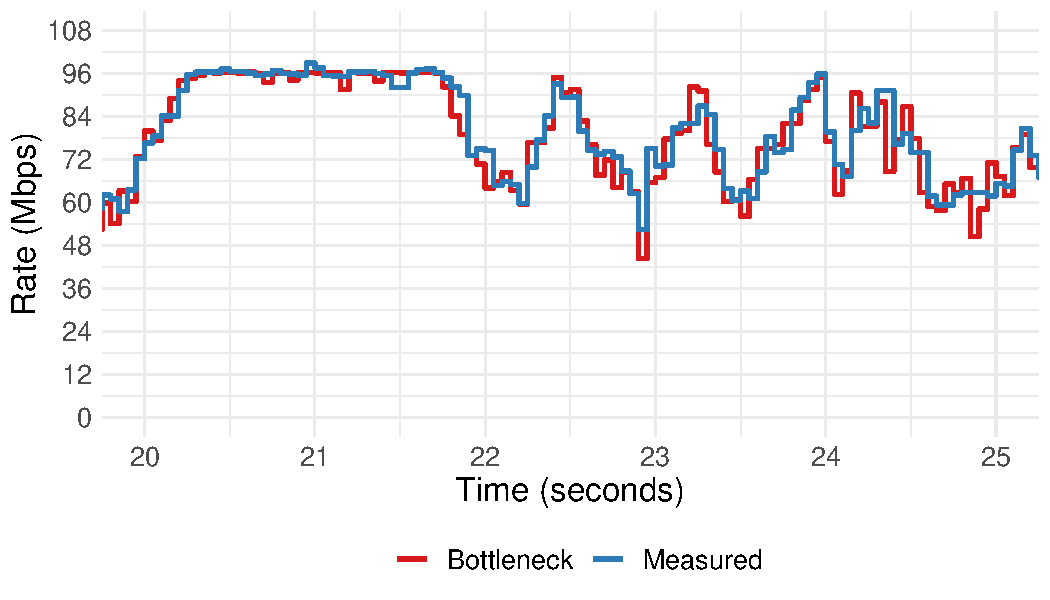
\includegraphics[width=\maxwidth]{figure/micro:time-thru-1} 

\end{knitrout}

    \caption{\name's estimate of the receive rate.}
    \label{fig:micro:time-thru}
\end{figure}
 % actually contains the time series
We now evaluate the accuracy of our measurement technique and its robustness to various network conditions. 

We pick 90 traces of \name's measurements from experiments in our evaluation across a range of RTTs (20ms, 50ms, 100ms) and bottleneck rates (24Mbps, 48Mbps, 96Mbps) and compute the difference between our measured value of the RTT and receive rate at each time step compared to the values at the bottleneck router. We plot the distribution of these differences for all of the traces in Figure~\ref{fig:micro:time-delay}. 80\% of our RTT estimates are within 1.2ms of the actual value and 80\% of our receive rate estimates are within 4Mbps of the actual value. 

To visualize how these measurements impact the behavior of the signals over time we pick an experiment for which the median difference matches that of the entire distribution and plot a five second segment of our estimates compared to the actual values in Figure~\ref{fig:micro:time-thru}.
\end{Appendix}
}